%
%\begin{itemize} 
%\item{ }
%A brief textual description of the overall flow diagram (along with its functional operation in the different user scenarios described in the first stage of the project).
%\item{ }
%A specification of each algorithm and associated data structures together with its entities, attributes, and operations ( include an English description of how they relate to your user scenario(s)).
%
%\end{itemize}
\begin{itemize} 
\item{  Short Textual Project Description. } \\
First, users input text(String), then we get the input and divide the input into words. \\
For each word, we firstly check if this word exists in our dictionary. If this word is in our dictionary, then this word is correctly spelled. If we cannot find this word in our dictionary, then this word is wrong. \\
For each wrong word, we first modify this word 3 times at most, if the modified word can be found in our dictionary, we give users a suggestion of modification. If we do not find any modified words within edit distance of 3 in our dictionary, we will tell users that we could not give any suggestion with respect to this word, and they should think about this word again carefully. \\
Overall average time complexity: $ O(\log n) $ for each operation, including lookup, insertion and deletion, where $ n $ stands for the number of nodes in the ternary search tree. \\
Overall space complexity: $ O(n) $, where $ n $ stands for the number of nodes in the ternary search tree, which is also the number of prefixes. 
E.g. there are 6 prefixes for word `trie' and `tree'(`t', `tr', `tre', `tree', `tri', `trie'). \\


\item{ Flow Diagram. }
\begin{figure}[H]
	\centering
	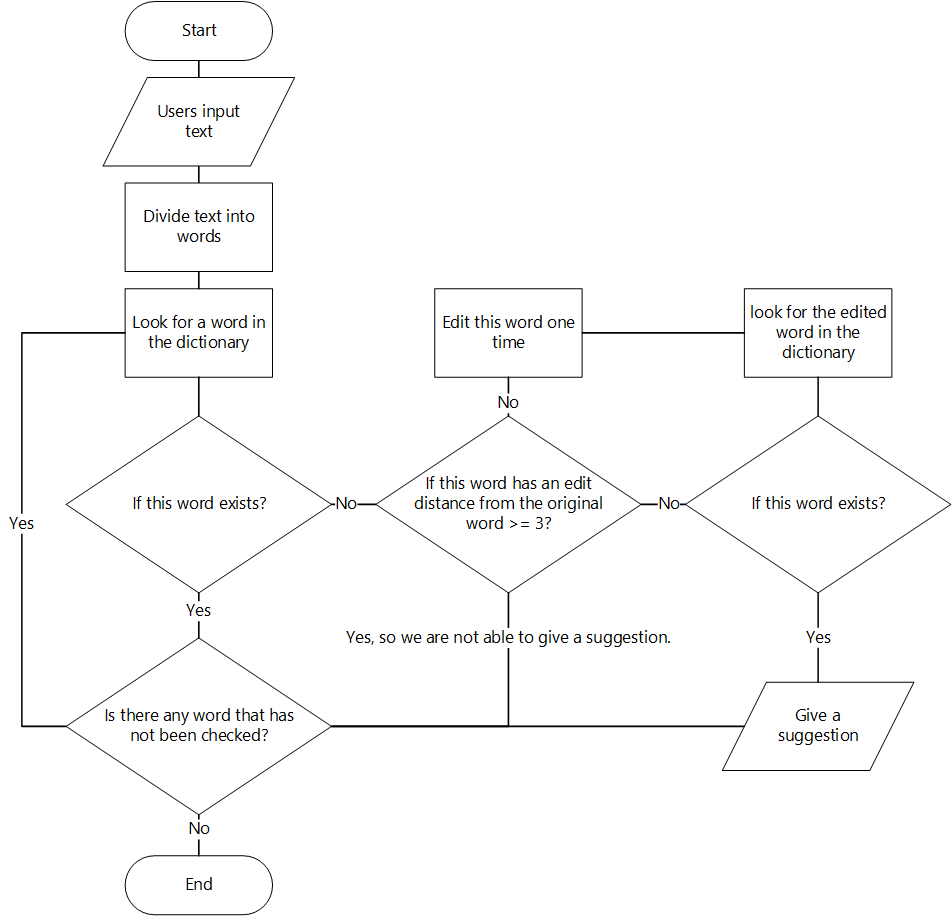
\includegraphics[width=0.5\textwidth]{fig/flow-diagram.png}
	\caption{Flow Diagram}
	\label{fig:flow-diagram}
\end{figure}
\item{ High Level Pseudo Code System Description. } \\
Pseudo codes are shown as follows.

\begingroup
\removelatexerror
\begin{algorithm}[H]
	\label{checkWord}
	\caption{checkWord}
	\KwData{Inputed text}
	\KwResult{Suggestions}
	split the input into words\;
	suggestions = an empty list of strings\;
	\ForEach{word in words}{
	suggestList = []\;
	\If{not checkDictionary(word)}{
		\For{i from 1 to 3}{
		\If{len(suggestList) $ > $ 5}{break;}
		editOneList = editDisOne(word)\;
		\ForEach{candidate in editOneList}{
			\If{len(suggestList) $ > $ 5}{break;}
			\If{checkDictionary (candidate)}{
				suggestList.append(candidate)\;
				suggestions[word] = suggestList\;
			}
		}
		}
	}
	}
	return suggestions\;
\end{algorithm}

\begin{algorithm}[H]
\label{checkDictionary}
\caption{checkDictionary}
\KwData{Word to be checked}
\KwResult{If this word is in dictionary}
	\eIf{word is in the ternary search tree}{
		return true;
	}{
		return false;
	}
\end{algorithm}

\begin{algorithm}[H]
\label{editDisOne}
\caption{editDisOne}
\KwData{Word to be edited}
\KwResult{A list of edited words}
splits = an empty list of pairs\;
deletes = an empty list of strings\;
transposes = an empty list of strings\;
replaces = an empty list of strings\;
inserts = an empty list of strings\;
result = an empty list of strings\;
\For{i from 1 to len(word) - 1}{splits.append([word(1, i), word(i + 1, len(word))])\;}
\ForEach{pair [a, b] in splits}{
	\If{len(b) $ > $ 1}{deletes.append(a + b(2, len(b)))\;}
	\If{len(b) $ > $ 2}{
		secondhalf = b(2, 2) + b(1, 1) + b(3, len(b))\;
		transposes.append(a + secondhalf)\;}
	\If{len(b) $ > $ 1}{
		\ForEach{letter in alphabet}{replaces.append(a + letter + b(2, len(b)))\;}
	}
	\ForEach{letter in alphabet}{replaces.append(a + letter + b(2, len(b)))\;}
}
put all candidates in deletes, transposes replaces and inserts into result\;
return result\;
\end{algorithm}
\endgroup

\item{Algorithms and Data Structures. } \\
In this project, we are using ternary search tree, which is a type of trie(or prefix tree). Compared to the 26-ary trie and binary tree, it has at most three children. So it's more space-efficient than trie. \\
Each node in ternary search tree stores a character, an indicator and up to three pointers pointing its children. The character is the data we stored. The indicator is a boolean value which tells us whether the node is the end of a word. The left child and the right child of the ternary seach tree act as the lowerbound and upperbound of prefix, help us easily find the prefix we actually want. \\
Ternary search tree supports tree operations: Insertion, search and deletion. The time complexity, as stated before, are $ O(\log n) $. \\
I also want to highlight the search operation. We process the string we want to search letter by letter. Everytime we try to look for only one letter in the ternary search tree. If the letter is equal to the character of current node, we move to the center child of current node and try to process next letter. If it is not, we move to the left or right child depending on the relation between the letter and the character of current node. The pseudo code is shown as Algorithm 4. \\
As Fig. 2 shows, it is a ternary search tree of word `TERNARY', `TREE', `TRIE' and `SEARCH'. 
\begin{figure}[H]
	\label{fig:tst}
	\centering
	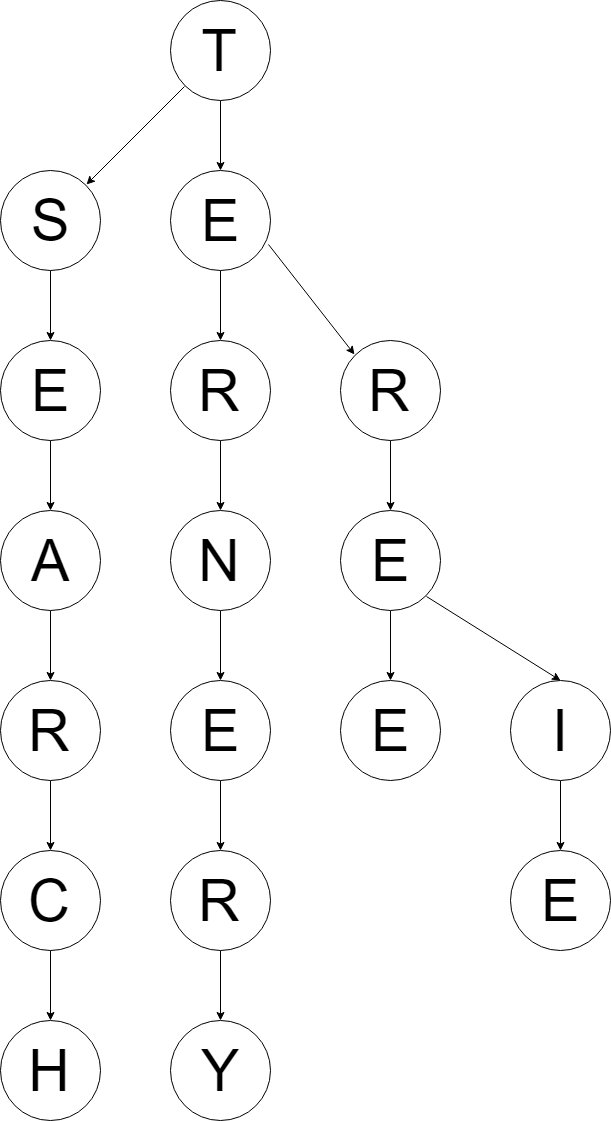
\includegraphics[height=0.3\textheight]{fig/TST.png}
	\caption{A ternary search tree}
\end{figure}

\begingroup
\removelatexerror
\begin{algorithm}[H]
	\label{search}
	\caption{Search in ternary search tree}
	\KwData{Word to be searched}
	\KwResult{Whether the search is successful}
	p $\gets$ the root of ternary search tree\;
	idx $\gets 0 $\;
	\While{p is not null}{
		\uIf{word[idx] $ < $ p.character}{
			p $\gets$ p.leftchild\;
		}
		\uElseIf{word[idx] $ > $ p.character}{
			p $\gets$ p.rightchild\;
		}
		\uElse {
			\If{idx == len(word) - 1 and p.indicator is true}{
				return true\;
			}
			idx $\gets$ idx + 1\;
			p $\gets$ p.centerchild
		}
	}
	return false\;
\end{algorithm}
\endgroup

\item{  Flow Diagram Major Constraints.}
Please insert here the integrity constraints:
\begin{itemize} 
\item{ Input Constraint: } \\
Description: In our project, we would check the spelling of English words, which means that the input must be English words, no matter if they are right or wrong. \\
Justification: All characters of each word inputed should be letters of alphabet. 
\end{itemize}
\end{itemize}

